\documentclass[11pt]{article}

\usepackage[margin=1in]{geometry}
\usepackage{amsmath,amssymb}
\usepackage{booktabs}
\usepackage{array}
\usepackage{graphicx}
\usepackage{float}
\usepackage{placeins}
\usepackage{hyperref}
\usepackage{xcolor}
\usepackage{enumitem}
\usepackage{microtype}
\usepackage{multirow}

\title{Sparse Cross-Document Contextualization for Persistent Native Memory\\
\large An Oracle Headroom Study beyond Packed RAG}
\author{Jorge Sim\~ao}
\date{Draft --- September 2026}

\newcommand{\pra}{\textsc{PRA}}
\newcommand{\rag}{\textsc{RAG}}

\begin{document}
\maketitle

\begin{abstract}
Retrieval-augmented generation (RAG) normally serializes selected documents into
one causal token sequence, so later documents are contextualized by earlier
documents before the query is decoded. Progressive Retrieval Attention (PRA)
instead allows selected resources to remain independently addressable and to
persist as native key/value memory. Prior work established that contiguous PRA
transport can preserve model behavior exactly, that pre-RoPE keys can be rebound
to request-specific packed positions, and that independently stored resources
closely reproduce a packed computation when document-to-document attention is
disabled. The remaining quality gap is therefore primarily a
cross-document-contextualization problem rather than a position-transport
problem.

This paper asks whether the useful portion of packed-RAG cross-document
interaction is sparse. We instrument the unchanged host-model attention path,
extract an oracle graph over physical layer/head/token edges, and replay the
same frozen retrieval selection under exact sparse masks. Candidate identities,
record order, prompt semantics, model revision, and generation settings remain
fixed. Compressed graphs retain only causal cross-record edges; immutable
selection receipts and graph digests tie every intervention to its source.

The inception experiment evaluates edge-count budgets from 0 to 100\% and
cumulative teacher-mass targets from 50 to 99\% on MultiHop-RAG. It also freezes
disjoint 2,000/150/150 train/validation/test identities for a possible learned
selector. On a ten-question mechanism cohort, 0.1\% of physical edges reached
.1488 F1 versus .1490 for packed RAG and .1431 for independent PRA, but this is
97.3\% recovery of a small 0.0059 gap and the cohort's packed official score was
only .600. We therefore run a powered 150-question frozen test comparing raw
attention with document-pair leave-one-group-out NLL, first-step JS, and a
finite-difference NLL-times-attention proxy. Pair NLL at 1\% obtains .1243 F1
and .3933 official score versus .1119 and .3333 for packed RAG; paired
differences are $+.0124$ F1 and $+.0600$ official, but both 95\% intervals
include zero. Every frontier remains non-monotonic and the absolute .19/.67
gate is missed. The result supports sparse causal headroom and shows that
task-aware rankings improve on raw magnitude, but it does not justify learned
selector training.

We then test a cheaper alternative: use one frozen selected record to retrieve
additional source intervals from another. Among 221 validation configurations,
dense selected-only expansion gains 2.94 support-span points using 12.66\%
extra native tokens, but recovers only 12.71\% of oracle headroom. Replayed
unchanged on 150 test questions, the gain contracts to 0.89 points and 95.3\%
of admitted tokens fall outside annotated support. Expansion-only native
generation lowers F1 from .0896 to .0761. Allowing attention only across
retrieval-linked record pairs restores F1 to .0874, statistically overlapping
independent PRA but not improving it. Cheap expansion finds some missing
evidence; current parameter-free scores do not select it precisely enough, and
cross-record interaction remains necessary to consume it safely.
\end{abstract}

\section{Introduction}

RAG systems solve a retrieval problem and a context-construction problem.
Retrieval selects useful evidence. Context construction then decides how that
evidence is presented to the language model. The common implementation packs
retrieved text into a causal sequence,
\[
D_1\,D_2\,\cdots\,D_m\,Q,
\]
and freshly prefills the whole sequence. This creates a dense and
order-dependent computation graph: $D_2$ can attend to $D_1$, $D_3$ can attend
to both $D_1$ and $D_2$, and the final query can attend to all preceding
states.

PRA exposes a different design point. Each $D_i$ can remain a persistent
addressable record with reusable model-native K/V. The query can later select
and materialize those records without rebuilding all source states. The
advantage is straightforward when a selection repeats or when records recur
across changing queries. The harder question is composition: independent
records do not contain the cross-document causal history introduced by ordinary
packed RAG.

Paper~3.2 localized this difference. Contiguous selected-context transport was
behaviorally exact across multiple model scales and families. Pre-RoPE
request-time rebinding reproduced the positional geometry of a packed request,
and independently encoded records closely tracked a packed control in which
document-to-document attention was disabled. In the powered natural comparison,
however, packed RAG remained stronger than independent PRA. A small trained
residual recovered part of the gap but did not establish a qualified solution.
Fixed sparse masks were non-monotonic, while one very small boundary interaction
budget approached packed F1 on some metrics.

These results motivate a narrower question:
\begin{quote}
\textbf{How much cross-document interaction is actually necessary, and can the
necessary interactions be predicted and executed sparsely at request time?}
\end{quote}

We therefore separate three quantities:
\begin{enumerate}[leftmargin=*]
    \item \textbf{persistent source state}, stored once as reusable PRA records;
    \item \textbf{request-specific interaction selection}, which determines
    which records/tokens/layers need contextualization;
    \item \textbf{request-specific interaction execution}, which applies a
    small amount of the frozen base model's own computation.
\end{enumerate}

The intended architecture is
\[
\begin{gathered}
\text{persistent PRA K/V}
\rightarrow
\text{sparse interaction selector}\\
\rightarrow
\text{small request-local cross-record computation}
\rightarrow Q.
\end{gathered}
\]

\paragraph{Contributions.}
This inception study makes four contributions:
\begin{enumerate}[leftmargin=*]
    \item A host-preserving attention observer and sparse-mask replay path that
    leaves base-model parameters and persistent records unchanged.
    \item A compressed physical-edge graph and immutable interaction-plan
    receipt spanning layers, heads, record pairs, and token positions.
    \item A prespecified oracle sparsification study over edge-count and
    cumulative-attention-mass budgets, with task and distribution metrics.
    \item A leakage-safe data split and an explicit learned pair-selector design
    that remains locked unless oracle evidence justifies training.
\end{enumerate}

\section{Related Work}

RAG and retrieval-conditioned language models place external evidence in the
model context or retrieve it during generation
\cite{lewis2020rag,guu2020realm,borgeaud2022retro}. Sparse-attention systems
reduce long-sequence cost through fixed, random, global, or learned access
patterns \cite{beltagy2020longformer,zaheer2020bigbird,roy2021routing}. Other
work retrieves external states at attention time or restricts K/V traffic
\cite{bertsch2023unlimiformer,tang2024quest,liu2025retrievalattention}. These
approaches motivate sparse access, but the present question is different: the
retrieved records are already selected and persist as independently encoded
native memory. We ask which request-specific cross-record interactions must be
restored to recover the behavior of a conventional packed prefix. CacheBlend
also studies reuse when separately cached chunks need request-time fusion
\cite{yao2024cacheblend}; our unit of intervention is an auditable physical
attention edge under a frozen RAG selection.

\section{Relationship to Prior PRA Work}

\subsection{Paper 1.5: request-time RoPE binding}

Paper~1.5 separated coordinate correctness from causal contextualization and
showed that, for RoPE models,
\[
K_{\mathrm{post}}(p)=R_pK_{\mathrm{pre}}.
\]
Pre-RoPE storage therefore allows a persistent key to be rebound to a
request-specific effective position without re-encoding the source.

Paper~3.3 assumes that positional contract and does not reopen the positional
transport question except as a runtime qualification requirement.

\subsection{Paper 3.0: materialization is a computational choice}

Paper~3.0 showed that more materialized K/V is not automatically better and
that useful detail depends on the query, evidence distribution, and consumer
layer. This motivates a query-conditioned interaction policy rather than a fixed
global cross-document mask.

\subsection{Paper 3.2: causal localization of the composition gap}

Paper~3.2 supplies the direct starting point. With a strong frozen selector,
packed RAG reached approximately .199 token F1 and .700 official score on the
final held-out comparison, while independent PRA reached approximately .135 and
.433. A rank-8 request-local residual raised PRA to approximately .154 F1 and
.533 official score but left substantial headroom and an uncertain five-seed
F1 effect.

More importantly, Paper~3.2 compared
\[
A=\text{full causal packed RAG},
\]
\[
B=\text{packed RAG with document-to-document attention disabled},
\]
and
\[
C=\text{independent pre-RoPE PRA records rebound to the same positions}.
\]
$B$ and $C$ were behaviorally close, while a shape-matched storage/rebinding
control was exact across the tested precision modes. The principal semantic
difference is therefore cross-document causal interaction.

Paper~3.3 does not attempt to make independent records reproduce every dense
packed state. It asks which subset of those interactions is needed for task
quality.

\section{Problem Formulation}

Let the selected evidence consist of $m$ persistent records
\[
\mathcal D=\{D_1,\ldots,D_m\},
\]
with total token count $T$. Let $\mathcal E_{\mathrm{full}}$ denote all
document-to-document attention edges allowed by ordinary packed causal RAG.

We seek a request-specific sparse edge set
\[
\mathcal E_q \subset \mathcal E_{\mathrm{full}}
\]
such that
\[
|\mathcal E_q| \ll |\mathcal E_{\mathrm{full}}|
\]
while preserving task utility:
\[
U(\mathcal D,Q,\mathcal E_q)
\approx
U(\mathcal D,Q,\mathcal E_{\mathrm{full}}).
\]

The system must additionally preserve most persistent native state:
\[
C_{\mathrm{new}}(\mathcal E_q)
\ll
C_{\mathrm{prefill}}(\mathcal D).
\]

Our primary quality target is to recover at least 80\% of the
independent-to-packed RAG gap under a request-specific interaction budget of at
most 10\% of dense cross-document interaction.

\section{Oracle Sparse Interaction}

\subsection{Teacher graph extraction}

We instrument packed RAG with frozen retrieval, reranking, selected records,
order, token budget, model, and generation settings. For every causal
document-to-document attention interaction we record sufficient metadata to
construct a sparse teacher graph:
\begin{itemize}[leftmargin=*]
    \item layer and head;
    \item source and target record/chunk;
    \item source and target token positions;
    \item attention mass;
    \item distance to document boundaries;
    \item retrieval rank and score.
\end{itemize}

Let $E$ be the set of causal token pairs whose source and target belong to
different records. The stored score array has shape $[L,H,|E|]$, not
$[L,H,T,T]$. Source and target token indices and record identities are stored
once, so within-record and causally impossible entries never enter the artifact.
For each layer, the observer computes probabilities on a diagnostic side path;
the hidden-state update still uses MLX's host scaled-dot-product-attention
kernel. A parity receipt checks the observer path against ordinary host
execution before the graph is interpreted.

\subsection{Oracle budgets}

We first retain the highest-attention edges at budgets
\[
0,\;0.01,\;0.05,\;0.1,\;0.5,\;1,\;2,\;5,\;10,\;100\%.
\]

A complementary cumulative-mass condition retains the smallest edge set
covering
\[
50,\;75,\;90,\;95,\;99\%
\]
of cross-document attention mass.

For replay, a plan contains a Boolean array of shape $[L,H,|E|]$. At layer
$\ell$, selected physical edges are added to a packed mask that otherwise
blocks cross-record attention. The frozen host model then executes the modified
mask. The 100\% plan must reproduce the packed teacher exactly; the 0\% plan
must reproduce the blocked packed control. These endpoint checks distinguish a
sparsification result from an instrumentation or transport error.

\subsection{Interventional ranking targets}

Attention magnitude is observational: a large coefficient shows that an
interaction occurred, not that it improved the answer. We therefore add a
leave-one-group-out utility for a group $g$,
\[
u_{\mathrm{NLL}}(g)
=
\mathcal L_{\mathrm{answer}}(M_{\setminus g})
-
\mathcal L_{\mathrm{answer}}(M),
\]
where $M$ is the packed teacher and $M_{\setminus g}$ removes only the group's
cross-document edges. A positive value means that removing the group raises
gold-answer NLL. We also measure first-step Jensen--Shannon divergence,
$u_{\mathrm{JS}}(g)$, between $M_{\setminus g}$ and $M$.

The hierarchy is document pair $\rightarrow$ layer $\rightarrow$ layer/head
$\rightarrow$ token edge. At each tested level, groups are ordered by measured
utility and physical edges within a group are refined by teacher attention. A
second pair-level proxy ranks by
\[
\max(0,u_{\mathrm{NLL}}(g))\,a_e,
\]
where $a_e$ is the teacher attention of edge $e$ in group $g$. This is a
finite-difference-times-attention diagnostic, not a gradient attribution.
These rankings are compared with raw attention at matched physical-edge
budgets $0,.01,.05,.1,.5,$ and $1\%$; 100\% remains an endpoint parity check.

Every natural question is sampled only after restricting the dataset to a
named frozen Paper~3.3 split. Atomic per-question checkpoints bind the dataset,
model, reranker, split digest, ranking targets, and budgets, so a resumed run
cannot mix configurations. A ten-question validation diagnostic localizes the
.1\% plans by layer, head, and document pair and selects ranking targets. The
powered confirmation then requires at least 100 previously untouched test
questions. Learned selection remains locked unless an interventional test
ranking meets the absolute quality gate and its F1 frontier is non-decreasing
through 1\%.

\subsection{Oracle gate}

The learned-selector program proceeds only if a sparse oracle can approach
packed-RAG quality. The initial gate is
\[
\mathrm{F1}\ge .19,
\qquad
\mathrm{official}\ge .67,
\]
or statistical indistinguishability from packed RAG while using no more than
5\% of dense cross-document interactions.

\section{Where Useful Interactions Live}

We analyze oracle-selected interactions by:
\begin{itemize}[leftmargin=*]
    \item transformer layer;
    \item attention head;
    \item source/target retrieval rank;
    \item document pair;
    \item chunk pair;
    \item token boundary distance;
    \item query overlap;
    \item entity/token overlap;
    \item gist similarity.
\end{itemize}

This analysis determines the appropriate routing granularity. If useful
interactions are largely pair-level, we avoid token-level prediction. If they
concentrate in a few layers or heads, request-local compute can be reduced
further.

\section{Learned Interaction Selection}

This section specifies the next-stage design; it is not evaluated in the
present paper. Training is deliberately locked by the failed inception gate.

\subsection{Pair selector}

The first learned policy predicts interaction importance for selected pair
$(D_i,D_j)$:
\[
s_{ij}=
f_\theta(g_q,g_i,g_j,r_i,r_j,\phi_{ij}),
\]
where $g_q$ is a query gist, $g_i,g_j$ are persistent record/chunk gists,
$r_i,r_j$ are retrieval/reranker features, and $\phi_{ij}$ contains pairwise
semantic features.

The pair selector is trained against oracle pair importance while controlling a
request-specific interaction budget.

\subsection{Layer/head selector}

If the oracle is concentrated, we extend the policy to
\[
s_{ij\ell h}
\]
or a factored approximation.

The paper prefers the simplest selector that reaches the quality/economics gate.

\section{Sparse Request-Local Contextualization}

Synthetic parameter-free K/V append failed in Paper~3.2. The present paper
therefore prioritizes on-manifold computation using the frozen base
transformer's own projections and attention operations.

Candidate mechanisms are:

\paragraph{Sparse packed-mask composition.}
Use selected interactions in a request-local composition pass as the first
oracle/runtime control.

\paragraph{Boundary interaction.}
Permit selected real boundary tokens to interact across selected record pairs.

\paragraph{Selected-token interaction.}
Use a learned token gate within selected record pairs.

\paragraph{Selected-layer propagation.}
Apply interaction only at selected layers, then propagate corrected request
states through the remaining decoder.

Persistent record K/V remains immutable. All corrections are request-local.

\section{Retrieval-Guided Cross-Document Expansion}

Physical-edge selection asks which neural interactions to replay. A cheaper
alternative asks an earlier question: whether one selected record identifies a
small, previously unselected interval in another selected record. Let
$S_i\subset D_i$ be the frozen first-stage span for record $D_i$. For every
allowed ordered pair $i\ne j$, we issue either
\[
S_i\longrightarrow \operatorname{search}(D_j)
\quad\text{or}\quad
(Q,S_i)\longrightarrow \operatorname{search}(D_j).
\]
The first form measures selected-span evidence alone; the second uses the user
query to suppress associations unrelated to the current reasoning path. Search
never escapes the records authorized by the frozen first-stage receipt.

We implement exact chunk BM25, frozen dense similarity, reciprocal-rank fusion,
an entity/keyterm channel, and a support-span oracle. Powered dense runs use
BAAI BGE-base-en-v1.5 with its query and document encodings kept distinct; the
dependency-free signed-hash encoder is an SDK fallback and is not labeled as a
semantic result. Dense vectors for authorized peer chunks, the request, and
selected source spans are prepared once per request. We report that preparation
separately from scorer latency so dense and fusion rows cannot inherit
order-dependent warm-cache advantages. For lexical rank
$r_{\mathrm{lex}}(c)$ and dense rank $r_{\mathrm{dense}}(c)$, the primary hybrid
score is
\[
s_{\mathrm{RRF}}(c)=
\frac{1}{60+r_{\mathrm{lex}}(c)}+
\frac{1}{60+r_{\mathrm{dense}}(c)}.
\]
RRF avoids calibrating unlike raw scores. A normalized weighted fusion is kept
as a secondary research arm. We also compare symmetric all-pairs expansion,
higher-to-lower and lower-to-higher retrieval rank, a top-record hub, and pairs
that pass a query-relevance threshold.

The runtime, rather than the search policy, owns safety and accounting. It
rejects unauthorized targets, removes overlap with the initial selection and
other expansions in logical source coordinates, clips the final interval to a
global token ceiling, and distinguishes resident from newly encoded native K/V.
For candidate set $C$ and admitted source intervals $A$, it records
\[
B_{\mathrm{cross}}\in\{32,64,128,256,512\},\qquad
k_{\mathrm{pair}}\in\{1,2,4,8\},
\]
together with requested, deduplicated, reused, and newly materialized tokens.
The hash-addressed \texttt{CrossDocumentExpansionReceipt} contains source and
target identities, offsets, channel scores, ranks, keyterms, policy revision,
and failure labels, but not raw source text.

Expansion and neural interaction remain separate interventions. \emph{Expansion
only} appends selected native source intervals without cross-record SA.
\emph{Pair SA} admits base-model attention only between retrieval-linked record
pairs. \emph{Boundary SA} further limits each linked pair to a source suffix and
target prefix. Finally, a diagnostic physical-edge arm ranks teacher edges only
inside retrieval-linked pairs. These masks execute through the unchanged host
attention implementation, so their edge fractions describe logical sparsity,
not kernel acceleration.

The public abstraction is fail-closed. Parameter-free modes have stable
configuration and plugin contracts, while oracle and weighted modes require an
explicit experiment flag. Runtime authorization, deduplication, budget
enforcement, and receipt generation also wrap custom plugins. No mode becomes
an SDK default from a smoke result: qualification requires a powered frozen
cohort, five-seed uncertainty, at least two model sizes, bounded quality and
latency, and preferably cross-family replication.

The first-stage selection cache stores tokenizer-independent source intervals
and checks the candidate receipt, selector identity, token ceiling, and record
limit before replay. Model tokenization occurs only during native encoding.
An interprocess receipt check during this work exposed two defects in the
historical BM25-v1 implementation: corpus term frequency had been accumulated
where document occurrence was required, and floating sums traversed an
unordered query-term set. BM25-v2 counts each term once per document and sorts
query terms before accumulation. We invalidated and regenerated all preliminary
expansion results after this correction; every new receipt carries the v2
revision. Earlier physical-edge results remain tied to their pinned historical
commit and are not silently relabeled as v2 comparisons.

\subsection{Frozen validation frontier}

We evaluate 221 policy configurations on 150 frozen validation questions. The
grid crosses five parameter-free channels and an oracle with selected-only or
query-conditioned probes, $k\in\{1,2,4,8\}$, and extra-native-token ceilings
from 32 to 512. Table~\ref{tab:expansion-validation} reports the best point per
channel subject to an extra-native fraction of at most 20\%. These are
validation choices, not test results. All non-oracle optima use a 64-token
ceiling, which is 12.66\% of the initial 506.2-token native selection on
average.

\begin{table}[t]
\centering
\small
\caption{Best bounded cross-document expansion point per channel on the
150-question validation split. Gains are absolute percentage points over the
same frozen first-stage selection. ``Q'' indicates query conditioning.}
\label{tab:expansion-validation}
\begin{tabular}{lcrrrrr}
\toprule
Channel & Q & Span gain & Chunk gain & Extra K/V & Distractor & Search ms \\
\midrule
Lexical & yes & 2.67 & 3.71 & 12.66\% & 90.00\% & 337.8 \\
Dense & no & \textbf{2.94} & 4.27 & 12.66\% & 86.00\% & 258.7 \\
RRF hybrid & yes & 2.44 & 3.79 & 12.66\% & 88.00\% & 344.7 \\
Weighted hybrid & yes & 1.83 & \textbf{4.35} & 12.66\% & 87.33\% & 340.5 \\
Entity/keyterm & yes & 1.72 & 2.71 & 12.66\% & 92.67\% & 337.0 \\
Oracle & yes & 23.17 & 30.55 & 19.65\% & 0.00\% & 338.2 \\
\bottomrule
\end{tabular}
\end{table}

Dense selected-only is the predeclared test policy: symmetric chunk search,
$k=1$, and a 64-token global ceiling. It raises supporting-span coverage from
41.33\% to 44.28\% and gold-chunk recall from 38.57\% to 42.85\%. Five repeated
paired bootstrap calculations place the span gain in a conservative
95\% interval of $[1.39,4.72]$ points and the chunk-recall gain in
$[2.51,6.22]$ points. Answer-string availability rises by 2.67 points,
with interval $[0.67,5.33]$.

The positive retrieval effect is not yet an efficiency or answer-quality win.
The selected policy requests 1,521.1 cross tokens per question before overlap
removal and global clipping, but admits only 64.0: a 23.77-fold
request-to-materialization amplification. Moreover, 86\% of admitted tokens do
not overlap annotated support. The compact oracle gains 23.17 span points with
99.4 extra tokens and no distractors; dense expansion therefore recovers only
12.71\% of oracle span headroom. Figure~\ref{fig:expansion-frontier} makes both
the bounded gain and the unresolved selectivity gap visible. Semantic vector
preparation adds 358.7 ms per request in this exhaustive research
implementation and is reported separately from the 258.7 ms dense search.

Direction and interval controls sharpen the diagnosis. Symmetric lexical
expansion gains 2.67 span points, whereas the query-selected-pair-only rule
gains 1.33 points while reducing the distractor fraction from 90.0\% to
38.7\% and the extra-native fraction from 12.66\% to 5.37\%. Restricting
deduplication to logical source intervals raises lexical chunk-recall gain to
6.96 points but does not close the oracle gap; the corresponding oracle gains
28.36 points with only 5.58\% extra native tokens. These controls show that
pair restriction and interval accounting can make expansion cleaner, but the
current parameter-free score still does not identify most missing support.

\begin{figure}[t]
\centering
\begin{minipage}{.49\linewidth}
\centering

\includegraphics[width=\linewidth]{../shared/results/paper3_3_crossdoc_expansion/validation_n150_bm25v2_semantic/support_gain_vs_cross_tokens.pdf}
\end{minipage}
\hfill
\begin{minipage}{.49\linewidth}
\centering

\includegraphics[width=\linewidth]{../shared/results/paper3_3_crossdoc_expansion/validation_n150_bm25v2_semantic/support_gain_vs_distractors.pdf}
\end{minipage}
\caption{Validation expansion frontier. Left: support-span gain against
additional native K/V. Right: gain against the fraction of admitted tokens
outside annotated support. Oracle points expose substantial unresolved
selection headroom.}
\label{fig:expansion-frontier}
\end{figure}
\FloatBarrier

\subsection{Frozen test retrieval}

We replay the validation-selected dense policy unchanged on the disjoint
150-question test split. Table~\ref{tab:expansion-test} includes two oracle
controls but does not use them to retune the policy. The locked policy raises
supporting-span coverage by 0.89 points, gold-chunk recall by 1.63 points, and
answer-string availability by 1.33 points. Conservative paired bootstrap
intervals are $[0.22,1.78]$, $[0.52,3.08]$, and $[0.00,3.33]$ points,
respectively. Thus the evidence-recovery effect transfers, but the
answer-availability interval touches zero.

\begin{table}[t]
\centering
\small
\caption{Frozen test retrieval. Oracle rows diagnose available headroom and
do not participate in policy selection.}
\label{tab:expansion-test}
\begin{tabular}{lrrrrrr}
\toprule
Condition & Span cov. & Chunk recall & Answer avail. & Extra K/V & Distractor & Tokens \\
\midrule
No expansion & 40.83 & 38.54 & 60.00 & 0.00\% & --- & 0.0 \\
Dense, 64 (locked) & 41.72 & 40.18 & 61.33 & 12.65\% & 95.33\% & 64.0 \\
Oracle, 64 & 50.67 & 64.48 & 60.00 & 9.00\% & 0.00\% & 45.6 \\
Oracle, 256 & 63.72 & 70.07 & 60.00 & 21.37\% & 0.00\% & 108.1 \\
\bottomrule
\end{tabular}
\end{table}

The matched 64-token oracle gains 9.83 span points and 25.93 chunk-recall
points while using fewer physical tokens than the dense policy. Dense
selected-only therefore recovers 9.04\% of matched-budget oracle span
headroom. Its 95.33\% distractor fraction also exceeds validation's 86.0\%.
This generalization gap keeps the parameter-free expansion policy
\texttt{RESEARCH\_ONLY}; the following generation experiment asks whether
the small retrieval gain nevertheless changes answer behavior.

\subsection{Native answer replay}

Table~\ref{tab:expansion-generation} replays the frozen test selection through
Qwen3-1.7B-4bit. The model sees 84.3 additional model-native tokens on average
after the 64 source-token intervals are tokenized. Expansion-only lowers F1
from .0896 for independent PRA to .0761 and official score from .4333 to
.3733. Its paired F1 effect is $-.0135$ with conservative 95\% interval
$[-.0272,.00005]$; the official-score effect is $-.0600$ with interval
$[-.1400,.0200]$. The interval endpoints prevent a directional significance
claim, but the means do not support promotion.

\begin{table}[t]
\centering
\small
\caption{Frozen 150-question Qwen3-1.7B native generation replay. Lower NLL is
better; times are per question in milliseconds. Linked masks execute a dense
host kernel and are mechanism controls, not sparse-speed results.}
\label{tab:expansion-generation}
\resizebox{\linewidth}{!}{%
\begin{tabular}{lrrrrrr}
\toprule
Condition & F1 & Official & Gold NLL & Encode & TTFT & Total \\
\midrule
Packed RAG & .0863 & .4267 & 5.3106 & 305.1 & 68.0 & 207.9 \\
Independent PRA & \textbf{.0896} & .4333 & 3.0310 & 362.2 & 75.0 & 214.1 \\
Expansion only & .0761 & .3733 & \textbf{2.6310} & 423.0 & 76.3 & 219.0 \\
Linked pair SA & .0874 & .4400 & 3.0117 & 808.2 & 71.4 & 214.8 \\
Linked boundary SA & .0879 & \textbf{.4467} & 3.0152 & 776.2 & 68.2 & 212.1 \\
Linked top-attention & .0783 & .3800 & 2.6583 & 775.5 & 68.2 & 211.6 \\
\bottomrule
\end{tabular}}
\end{table}

Retrieval-linked pair SA reduces the expansion-only F1 deficit relative to
independent PRA by 84.1\%; the boundary variant reduces it by 87.6\%. Their
remaining paired F1 effects, $-.0021$ and $-.0017$, have intervals
$[-.0099,.0056]$ and $[-.0111,.0081]$. Both linked modes are therefore
statistically compatible with independent PRA on this cohort, not superior to
it. The apparently favorable expansion-only gold NLL is especially
instructive: it improves by .4000 while decoded F1 and official score decline.
Answer-likelihood distillation alone would select the wrong deployment policy.

\begin{figure}[t]
\centering

\includegraphics[width=.96\linewidth]{../shared/results/paper3_3_crossdoc_expansion/generation_test_qwen17b_dense64/generation_quality.pdf}
\caption{Absolute answer F1 and official MultiHop-RAG score for the frozen
Qwen3-1.7B replay. Error bars are conservative envelopes across five paired
bootstrap calculations; they do not represent independently trained models.}
\label{fig:expansion-generation}
\end{figure}
\FloatBarrier

\paragraph{Gold-support expansion oracle.}
The matched 64-source-token oracle separates routing error from consumption.
It adds 60.1 model-native tokens on average and raises retrieval support-span
coverage by 9.83 points, yet expansion-only F1 falls from .0896 to .0829
($-.0066$, 95\% interval $[-.0170,.0037]$) and official score falls from
.4333 to .4000 ($-.0333$, interval $[-.0933,.0267]$). Linked pair SA restores
F1 to .0888 and boundary SA to .0895; both overlap independent PRA. The packed
endpoint is already slightly below independent PRA on this cohort, so a
packed-gap-recovery ratio is not meaningful. More importantly, even correctly
identified missing support does not improve absolute answer quality when it is
merely appended as independently encoded native memory. The mechanism gate is
therefore closed for both parameter-free and oracle expansion-only execution.

\subsection{Reduced scale and family replication}

We replay the identical selection-cache digest on 30 matched test questions
with Qwen3-4B, Qwen3-8B, and Llama-3.1-8B-Instruct. These reduced cohorts test
directional transfer; they do not have the power of the 150-question 1.7B run.
Table~\ref{tab:expansion-ladder} reports paired percentage-point effects
against each model's independent-PRA condition.

\begin{table}[t]
\centering
\small
\caption{Model ladder effects versus independent PRA. Columns report F1
changes for the three interventions and the expansion-only official-score
change.}
\label{tab:expansion-ladder}
\begin{tabular}{lrrrrr}
\toprule
Model & $n$ & Expansion F1 & Pair-SA F1 & Boundary F1 & Expansion official \\
\midrule
Qwen3-1.7B & 150 & $-1.35$ & $-0.21$ & $-0.17$ & $-6.00$ \\
Qwen3-4B & 30 & $+0.64$ & $-1.31$ & $-0.65$ & $-3.33$ \\
Qwen3-8B & 30 & $-0.03$ & $+0.92$ & $+0.81$ & $-3.33$ \\
Llama-3.1-8B & 30 & $+2.78$ & $-3.39$ & $-4.85$ & $+3.33$ \\
\bottomrule
\end{tabular}
\end{table}

No intervention has a consistent sign across scale and family. The only F1
interval excluding zero is the negative Qwen3-4B pair-SA effect,
$[-2.83,-0.09]$ points. Llama expansion-only has the largest positive mean,
but its interval is $[-8.42,13.73]$ points; the corresponding official-score
interval is $[0,10]$ points. Qwen3-8B pair SA is directionally positive but
also uncertain. These results reject a universal larger-model consumption
claim and keep both expansion and linked attention outside the SDK default
surface.

\begin{figure}[t]
\centering
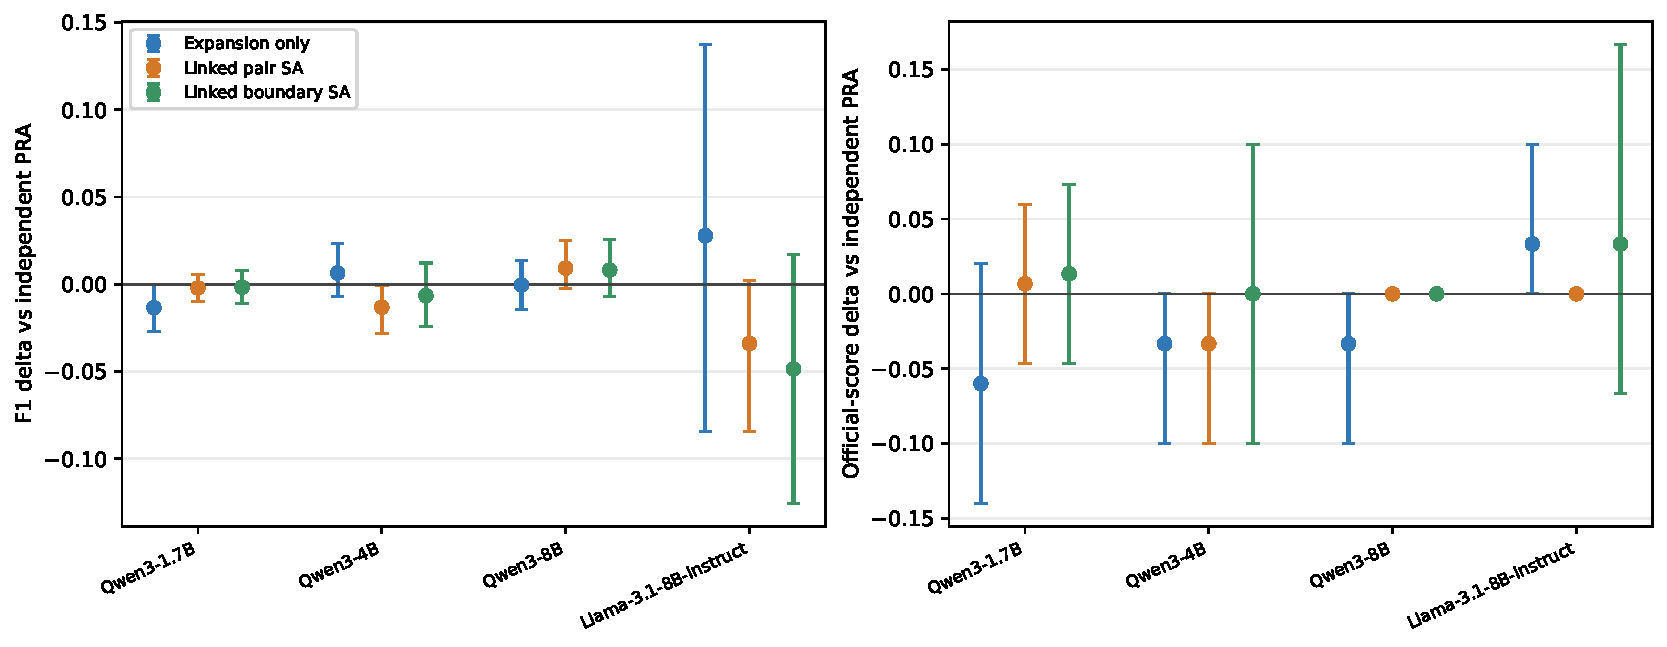
\includegraphics[width=.96\linewidth]{../shared/results/paper3_3_crossdoc_expansion/model_ladder_dense64/model_ladder_effects.pdf}
\caption{Paired generation effects across model scale and family. Error bars
are conservative bootstrap envelopes. The 1.7B point uses 150 questions; the
three qualification points use the same 30-question subset.}
\label{fig:expansion-ladder}
\end{figure}
\FloatBarrier

\subsection{SDK qualification decision}

Table~\ref{tab:expansion-sdk-gate} applies the predeclared SDK gate. The
implementation itself is reproducible and auditable, but neither dense
expansion nor linked SA has a stable answer-quality advantage.

\begin{table}[H]
\centering
\small
\caption{Cross-document expansion SDK qualification.}
\label{tab:expansion-sdk-gate}
\begin{tabular}{>{\raggedright\arraybackslash}p{.40\linewidth}>{\raggedright\arraybackslash}p{.40\linewidth}>{\raggedright\arraybackslash}p{.09\linewidth}}
\toprule
Criterion & Result & Gate \\
\midrule
Pinned deterministic policy and immutable receipt & BGE revisions and cache digest recorded & Pass \\
No test-set tuning & Validation-selected policy replayed unchanged & Pass \\
At most 20\% extra native K/V & 12.65\% source-token fraction on test & Pass \\
At least 50\% packed-gap F1 recovery & No positive packed gap; expansion lowers 1.7B F1 & Fail \\
No meaningful quality regression & Negative 1.7B mean; inconsistent ladder & Fail \\
Independent-seed stability & Bootstrap resampling only, not five model runs & Not met \\
Bounded production latency & 370.3 ms preparation plus 249.5 ms exhaustive search & Not met \\
Two sizes and cross-family check & Qwen 1.7B/4B/8B and Llama 8B & Pass \\
Authorization, fallback, and audit receipt & Fail-closed runtime tests & Pass \\
\bottomrule
\end{tabular}
\end{table}

The stable public behavior remains \texttt{mode=none}. Expansion modes remain
explicit research options, oracle access remains experiment-only, and
iteration depth two stays rejected by validation until one-pass quality
qualifies. A learned selector is likewise not unlocked: the failure now
includes consumption of an oracle selection, not merely a weak
parameter-free ranker.

\section{Training Objective}

The base model remains frozen initially.

We optimize
\[
\mathcal L =
\lambda_{\mathrm{task}}\mathcal L_{\mathrm{answer}}
+
\lambda_{\mathrm{seq}}
KL(P_{\mathrm{sparse}}\Vert P_{\mathrm{packed}})
+
\lambda_{\mathrm{sel}}\mathcal L_{\mathrm{selector}}
+
\lambda_{\mathrm{cost}}C_{\mathrm{interaction}}.
\]

Task quality receives the dominant weight. Global K/V reconstruction is not a
primary objective because Paper~3.2 showed that state proximity, answer NLL,
and generated-answer quality need not agree.

\section{Order Robustness}

Packed RAG changes its causal graph when selected documents are permuted. PRA
records offer the possibility of more stable set-like evidence composition.

We evaluate canonical, reverse, and random permutations under:
\begin{itemize}[leftmargin=*]
    \item packed RAG;
    \item independent PRA;
    \item oracle sparse composition;
    \item learned sparse composition.
\end{itemize}

We report task quality together with mean pairwise JS, unique outputs per
question, and F1/NLL variance. Lower order sensitivity is considered a benefit
only at matched or improved task quality.

\section{Experimental Protocol}

\subsection{Dataset}

MultiHop-RAG is the first mandatory dataset because Paper~3.2 already provides
frozen retrieval, canonical records, support labels, and powered natural
baselines.

Additional datasets are introduced only after the mechanism passes the primary
gate.

\subsection{Selection}

Use the strongest qualified matched selector from Paper~3.2:
\[
\mathrm{BM25}\rightarrow\mathrm{BGE\mbox{-}v2\mbox{-}M3}.
\]

Candidate and selection receipts are frozen before composition conditions run.

\subsection{Training split}

The frozen split uses:
\begin{itemize}[leftmargin=*]
    \item 2,000 training questions;
    \item 150 validation questions;
    \item 150 fixed held-out test questions; paired uncertainty uses
    bootstrap seeds 11, 23, 37, 71, and 101, which are repeated resampling
    calculations rather than independent model runs.
\end{itemize}

The split seed is 3301. All 30 identities declared by the final Paper~3.2
rank-8 residual manifest are excluded from every Paper~3.3 split, rather than
only from training. The dataset revision, corpus revision, exact identities,
legacy manifest, and split digest are persisted. Oracle smoke questions do not
train or select parameters.

\subsection{Model ladder}

\begin{description}[leftmargin=2cm]
    \item[M0] Qwen3-1.7B: full discovery/training matrix.
    \item[M1] Qwen3-4B: reduced qualification.
    \item[M2] Qwen3-8B: reduced qualification.
    \item[M3] Llama-3.1-8B: cross-family qualification.
\end{description}

\section{Baselines}

Mandatory baselines:
\begin{enumerate}[leftmargin=*]
    \item packed RAG;
    \item independent pre-RoPE PRA;
    \item Paper~3.2 rank-8 residual;
    \item fixed sparse boundary mask;
    \item oracle sparse interaction;
    \item learned sparse selector/composer.
\end{enumerate}

\section{Metrics}

\paragraph{Task quality.}
Official score, token F1, exact match, gold-answer NLL, and answer
log-probability.

\paragraph{Distributional fidelity.}
First-step JS/KL, logit differences, and generated-output agreement.

\paragraph{Sparsity.}
Selected document pairs, layers, heads, tokens, and total cross-document
interaction edges.

\paragraph{Systems.}
Persistent K/V reuse, newly computed states, request-local FLOPs, composition
latency, TTFT, total latency, and memory.

\paragraph{Robustness.}
Five-seed intervals, order sensitivity, model-scale transfer, family transfer,
and precision sensitivity.

\section{Inception Results}

\subsection{Scope and endpoint validity}

We ran the complete oracle grid on ten deterministically selected MultiHop-RAG
questions with Qwen3-1.7B-4bit on an Apple M4 Pro with 48~GiB unified memory.
BM25 produced 20 candidates, BGE-v2-M3 reranked them, and a 512-token budget
retained three or four records. The model, reranker, corpus, and dataset
revisions are pinned in the manifest. This is a one-seed mechanism cohort, not
a population estimate. A post-freeze provenance check places all ten identities
in the Paper~3.3 training partition, with no overlap with the Paper~3.2 final
evaluation identities. The validation diagnostic and powered test confirmation
therefore remain disjoint from this inception result.

Observer instrumentation matched ordinary host execution on all 10 questions.
The 100\% physical-edge plan also matched the instrumented packed teacher on all
10, with zero K/V delta and zero first-step JS. The 0\% plan matched the packed
no-cross-document mask. The average teacher graph contained 38.04 million
physical cross-document edges over 28 layers and 16 heads. These checks close
the implementation gate: differences inside the sweep are caused by the edge
mask, not by an alternate attention kernel.

\subsection{Quality--sparsity frontier}

\begin{table}[ht]
\centering
\small
\caption{Paper 3.3 oracle smoke. ``Edges'' is the fraction of physical
layer/head/token-pair cross-document edges. Attention mass is measured under
the packed teacher.}
\label{tab:oracle-frontier}
\begin{tabular}{lrrrrr}
\toprule
Condition & F1 & Official & Gold NLL & Edges & Mass \\
\midrule
Packed host / oracle 100\% & .1490 & .600 & 4.780 & 100\% & 100\% \\
Independent PRA & .1431 & .600 & 2.550 & 0\% & 0\% \\
Oracle top 0.01\% & .1449 & .600 & 2.579 & .01\% & 4.0\% \\
Oracle top 0.05\% & .1416 & .600 & 2.571 & .05\% & 19.2\% \\
Oracle top 0.1\% & \textbf{.1488} & \textbf{.600} & 2.610 & .1\% & 36.2\% \\
Oracle top 0.5\% & .0968 & .400 & 4.794 & .5\% & 80.3\% \\
Oracle top 5\% & .0990 & .400 & 4.851 & 5\% & 91.9\% \\
Oracle top 10\% & .1212 & .500 & 4.852 & 10\% & 95.1\% \\
\midrule
Mass oracle 50\% & .1403 & .500 & 2.753 & .149\% & 50\% \\
Mass oracle 75\% & .1145 & .500 & 3.757 & .324\% & 75\% \\
Mass oracle 90\% & .0768 & .400 & 4.758 & 3.466\% & 90\% \\
Mass oracle 99\% & .1308 & .500 & 4.855 & 30.902\% & 99\% \\
\bottomrule
\end{tabular}
\end{table}

At 0.1\% physical edges, the oracle recovers 97.3\% of this ten-question
cohort's small 0.0059 F1 packed--independent gap: F1 is .1488 versus .1490 for
packed RAG and .1431 for independent PRA. Official score remained .600 in all
three conditions, so no official-score gap existed to recover. The 0.1\% plan
did not reproduce the same strings as packed RAG: output agreement was 0/10 and
first-step JS remained .110. The result is therefore task-level headroom, not
behavioral equivalence, and the relative percentage should not be read as a
large absolute quality gain.

The frontier is strongly non-monotonic. Increasing the top-edge budget from
0.1\% to 0.5\% reduced F1 from .1488 to .0968 even though retained teacher mass
rose from 36.2\% to 80.3\%. Likewise, the smallest set carrying 50\% of teacher
mass used only .149\% of physical edges but did not outperform independent PRA.
Raw attention mass is thus an inadequate causal-utility target by itself.

\begin{figure}[ht]
\centering

\includegraphics[width=.86\linewidth]{../shared/results/paper3_3_sparse_crossdoc/oracle_natural_seed11_n10/oracle_quality_frontier.pdf}
\caption{Task quality and retained teacher mass across physical top-edge
budgets. The curve is a mechanism smoke over ten questions; connecting lines do
not imply monotonicity or statistical precision.}
\label{fig:oracle-frontier}
\end{figure}

\subsection{Interaction localization}

Cross-document attention mass was distributed across the network: layers
0--8 contained 27.4\%, layers 9--18 contained 31.7\%, and layers 19--27
contained 40.8\%. No single layer exceeded 4.85\% on average, and the largest
layer/head cell averaged only .357\%. The graph is therefore late-leaning but
not localized to one layer or head. Pair mass was more concentrated: the first
record supplied 49.1\% of mass into the second and 38.8\% into the third.
These values partly reflect causal geometry and token counts; they are routing
features to test, not evidence that early-ranked records are causally sufficient.

\begin{figure}[ht]
\centering

\includegraphics[width=.78\linewidth]{../shared/results/paper3_3_sparse_crossdoc/oracle_natural_seed11_n10/oracle_layer_localization.pdf}
\caption{Mean share of packed-teacher cross-document attention mass by decoder
layer. Later layers carry more aggregate mass, but no narrow layer band
dominates.}
\label{fig:layer-localization}
\end{figure}

\subsection{Interventional validation}

We next ran the six ranking targets on ten frozen validation questions, using
the same model, selector, 512-token budget, and physical-edge replay. The BGE
reranker ran on MPS; this execution device is part of the run configuration and
receipt. All ten ordinary/instrumented host comparisons and all ten 100\%
replay checks passed exactly.

\begin{table}[ht]
\centering
\small
\caption{Frozen validation target selection. Each oracle row reports its
highest-F1 budget at or below 1\%; it is not a test-set estimate.}
\label{tab:interventional-validation}
\begin{tabular}{lrrrr}
\toprule
Condition & Edges & F1 & Official & Gold NLL \\
\midrule
Packed teacher & 100\% & .1094 & .600 & 5.911 \\
Independent PRA & 0\% & .1673 & .500 & 3.211 \\
Raw attention & .1\% & .1706 & .500 & 3.697 \\
Pair NLL & 1\% & .1659 & .600 & 3.929 \\
Pair JS & .5\% & \textbf{.1727} & .600 & 3.666 \\
Pair NLL $\times$ attention & .1\% & .1379 & .400 & 3.861 \\
Layer NLL & .01\% & .1540 & .400 & 3.204 \\
Layer JS & .5\% & .1525 & .500 & 3.739 \\
\bottomrule
\end{tabular}
\end{table}

This cohort reverses the inception endpoint: independent PRA exceeds packed
F1 by .0579, although packed retains .100 more official score. It therefore
does not define a packed advantage that sparse edges can meaningfully recover.
The apparent improvements are also uncertain. Relative to the packed teacher,
pair-JS at .5\% changes F1 by $+.0633$ (paired bootstrap 95\% interval
$[-.0067,.1618]$) with zero mean official-score change; raw attention at .1\%
changes F1 by $+.0613$ ($[-.0275,.1604]$) while changing official score by
$-.100$. Both intervals include zero. Gold NLL ranks conditions differently
from generated-answer metrics, so lower teacher-forced loss is not treated as
proof of better task behavior.

No ranking has a non-decreasing F1 frontier through 1\%. The result therefore
strengthens, rather than resolves, the inception warning: raw magnitude is not
a causal utility signal, and coarse leave-one-group-out NLL or first-step JS is
not sufficient by itself. The powered test carries raw attention, pair NLL,
pair JS, and pair-NLL-times-attention forward. Layer-only policies are dropped
after validation because they do not improve the quality frontier.

\subsection{Powered frozen-test confirmation}

We then evaluate all 150 previously untouched test identities. The model is
Qwen3-1.7B-4bit on an Apple M5 with 16~GiB unified memory; the BGE reranker runs
on MPS. All 150 ordinary/instrumented comparisons and all 150 full-replay
comparisons pass exactly. The run takes 18,486 seconds and records 4,800
condition rows. Table~\ref{tab:powered-oracle} reports the highest-F1 point at
or below 1\% for each ranking. These are test-set summaries selected over a
small prespecified budget grid, not independently tuned deployment settings.

\begin{table}[ht]
\centering
\small
\caption{Powered 150-question frozen test. Oracle rows show the best F1 budget
at or below 1\% physical cross-document edges.}
\label{tab:powered-oracle}
\begin{tabular}{lrrrr}
\toprule
Condition & Edges & F1 & Official & Gold NLL \\
\midrule
Packed teacher & 100\% & .1119 & .3333 & 5.526 \\
No-cross-document packed & 0\% & .1105 & .3600 & 3.097 \\
Independent PRA & 0\% & .1129 & .3667 & 3.114 \\
Raw attention & .05\% & .1148 & .3867 & 3.100 \\
Pair JS & 1\% & .1205 & .3800 & 3.817 \\
Pair NLL & 1\% & \textbf{.1243} & .3933 & 3.675 \\
Pair NLL $\times$ attention & .1\% & .1215 & \textbf{.4000} & 3.319 \\
\bottomrule
\end{tabular}
\end{table}

Pair NLL at 1\% changes F1 by $+.0124$ relative to packed RAG (paired bootstrap
95\% interval $[-.0055,.0315]$) and official score by $+.0600$
($[-.0133,.1333]$). The combined proxy at .1\% changes F1 by $+.0096$
($[-.0078,.0289]$) and official score by $+.0667$
($[-.0067,.1400]$). Pair JS at 1\% and raw attention at .05\% also have intervals
spanning zero. The powered result therefore distinguishes mean frontier shape
from established superiority: causal grouping produces the better sparse
means, but no task-quality effect is conclusive.

The endpoint ordering is itself informative. Packed F1 differs from independent
PRA by only $-.0010$, and its paired interval includes zero. Gold NLL strongly
prefers the blocked and independent conditions, so NLL divergence from packed
does not translate monotonically into generated-answer quality. This cohort
cannot support a claim that dense packed contextualization is a better task
endpoint than a sparse oracle merely needs to recover.

\begin{figure}[ht]
\centering
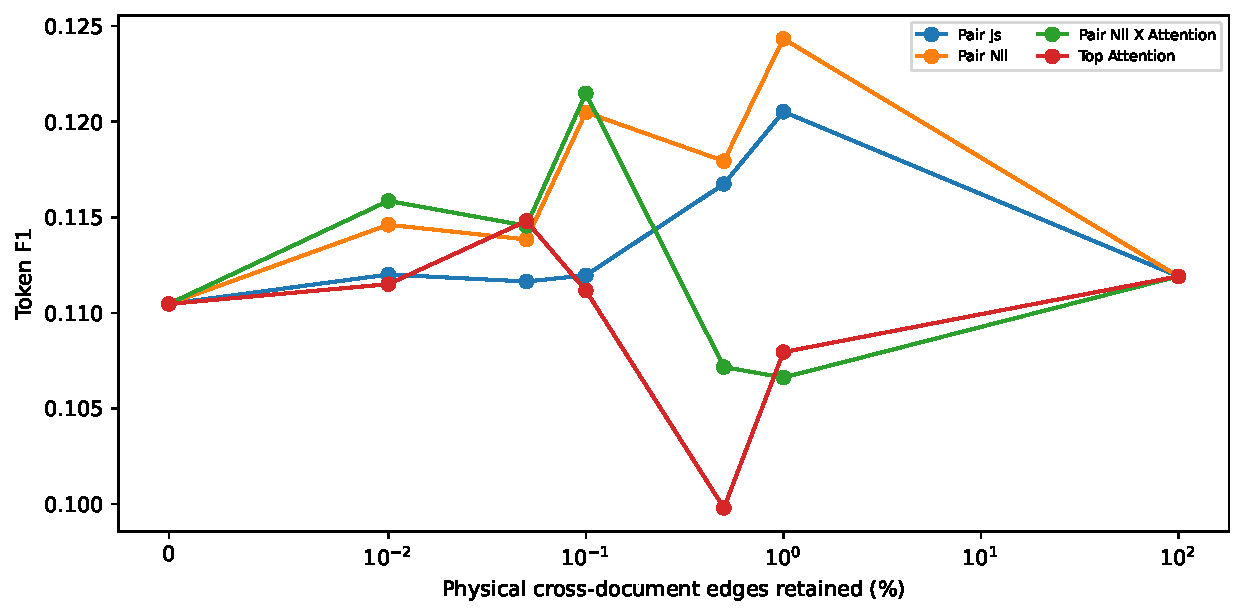
\includegraphics[width=.88\linewidth]{../shared/results/paper3_3_sparse_crossdoc/interventional_test_n150/ranking_target_frontiers.pdf}
\caption{Powered-test F1 frontiers for observational and interventional
rankings. Causal pair rankings improve the mean sparse frontier, but all curves
remain non-monotonic; lines aid reading and do not imply interpolation.}
\label{fig:powered-frontiers}
\end{figure}

The powered .1\% plans also reveal different geometries. Raw attention assigns
32.6\% of edges to layers 23--25 and 27 and 94.3\% to pairs $(0,1)$ and $(0,2)$.
Pair NLL spreads 84.8\% across $(0,2)$, $(1,2)$, and $(0,1)$ and emphasizes
early layers 1--2 alongside distributed later layers. Pair JS assigns 86.7\%
to $(0,1)$, while the combined proxy assigns 91.7\% across the first three
pairs and leans later. No leading layer--head cell receives more than .86\% of
a policy's selected edges. These are policy-induced concentrations, not
universal heads, but they show that the causal target materially changes the
proposed sparse computation.

\begin{figure}[ht]
\centering
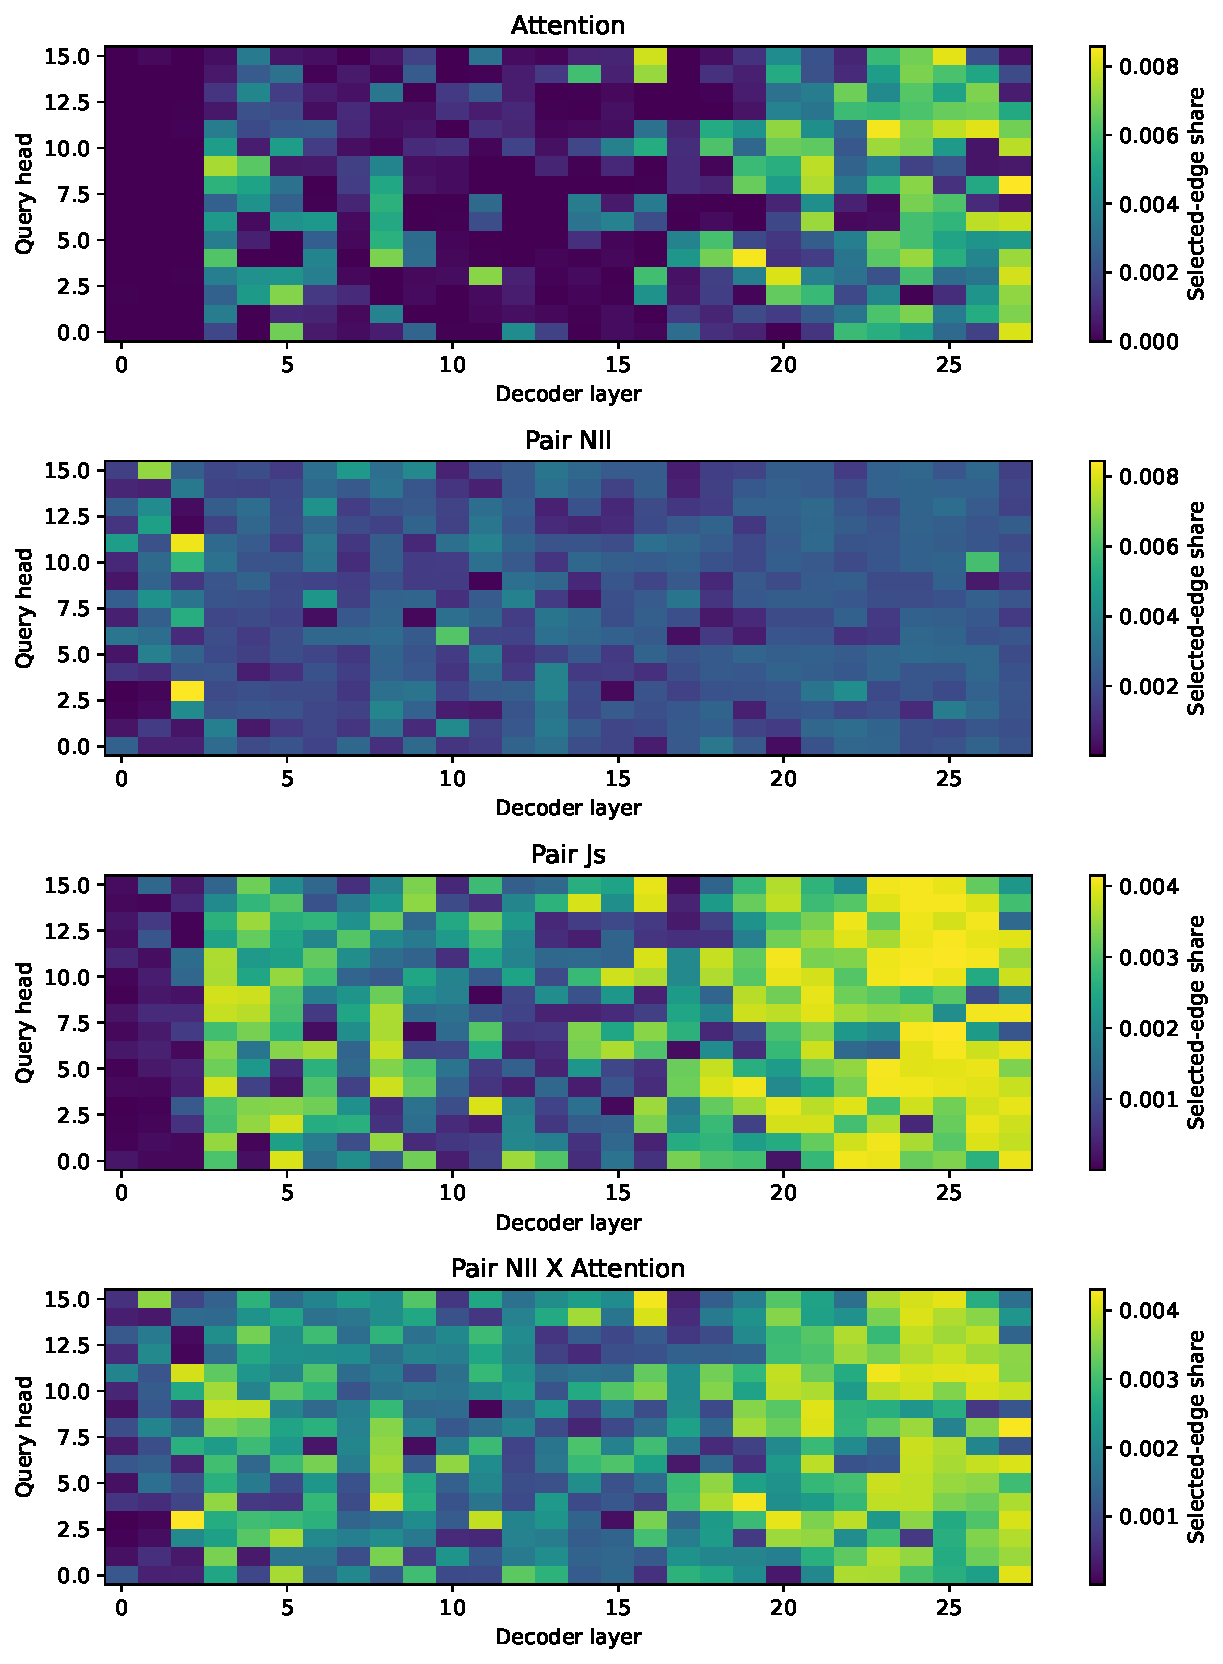
\includegraphics[width=.92\linewidth]{../shared/results/paper3_3_sparse_crossdoc/interventional_test_n150/selected_edge_layer_head.pdf}
\caption{Layer--head allocation of each .1\% plan over 150 frozen test
questions. Color is selected-edge share within a policy.}
\label{fig:selected-edge-localization}
\end{figure}
\FloatBarrier

\subsection{Go/no-go decision}

The powered gate is \textbf{locked}. The cohort-size requirement is met, but no
condition reaches .19 F1 and .67 official score, no frontier is non-decreasing
through 1\%, and the paired task-quality intervals include zero. Learned
selector training therefore remains disabled. The next useful selector target
must improve causal localization beyond one scalar utility per document pair;
training the current target would turn an unresolved oracle into a learned
approximation of an unstable policy.

The reported encoding times, roughly 0.5--0.9 seconds per condition, execute a
dense host attention kernel under a sparse mask. Edge fraction is therefore a
logical interaction budget, not a measured wall-time or FLOP reduction. A
production sparse kernel is downstream work and should be evaluated only after
the quality gate passes.

\section{Success Criteria}

The predeclared practical gate is
\[
\mathrm{F1}\ge .19,
\qquad
\mathrm{official}\ge .67,
\]
or statistical indistinguishability from packed RAG, while using no more than
5\% of dense request-specific cross-document interaction. Approximate 80\%
gap recovery remains a useful descriptive quantity, but does not replace these
absolute thresholds.

Neither the ten-question smoke nor the 150-question frozen test meets these
absolute criteria. The smoke's 0.1\% point meets the relative F1-recovery target
only because its packed and independent endpoints are close. On the powered
test, causal rankings improve sparse mean quality but do not establish a
monotonic frontier or a nonzero paired task-quality effect. We do not substitute
either post-hoc observation for the prespecified gate.

Retrieval-guided expansion also misses its separate promotion gate. The locked
policy recovers evidence at a bounded token cost, but expansion-only generation
does not recover 50\% of a packed-RAG F1 gap or avoid a negative 1.7B mean.
The gold-support oracle shows that improving the router alone is insufficient.

A stronger result matches packed RAG within uncertainty while preserving:
\begin{itemize}[leftmargin=*]
    \item persistent native K/V reuse;
    \item lower order sensitivity;
    \item materially lower request-specific compute.
\end{itemize}

\section{Falsification}

Scientifically useful negative outcomes include:
\begin{itemize}[leftmargin=*]
    \item an oracle requires dense interaction;
    \item learned selection fails to approach the oracle;
    \item sparse state propagation destroys quality;
    \item selector overhead erases saved prefill;
    \item order robustness disappears at matched quality;
    \item the mechanism does not transfer across models/families.
\end{itemize}

\section{Systems Integration}

Paper~3.3 reuses the canonical Paper~4.5/Paper~3.2 \texttt{ContextRecord} and storage
metadata. The learned interaction policy is request-local and must not mutate
persistent source records.

The target runtime abstraction is
\[
\texttt{ContextRecord}
\rightarrow
\texttt{SelectionReceipt}
\rightarrow
\texttt{InteractionPlan}
\rightarrow
\texttt{RequestLocalComposition}.
\]

An \texttt{InteractionPlan} should record selected record pairs, token spans,
layers/heads, budget, policy revision, and model/runtime compatibility.

\section{Discussion}

The 0.1\% result suggests that conventional RAG may perform substantially
redundant document-to-document computation. It does not yet establish that
claim: the sample is small, the absolute gate failed, and the present sparse
mask still executes a dense kernel. PRA could eventually retain persistent
source state and pay only for a small request-specific neural ``join'' among
selected resources, but that economic claim requires both powered quality and
a real sparse execution path.

Retrieval-guided expansion gives a more concrete decomposition. Its
parameter-free router finds a statistically positive but small amount of
missing support, with poor precision. Replacing it with a support oracle
substantially improves evidence recovery but still does not improve
expansion-only answers. Retrieval-linked pair or boundary attention then
restores much of the lost quality. The sequence locates two distinct research
problems: selecting useful peer intervals and contextualizing those intervals
without rebuilding a dense packed prefix. Neither can be inferred from gold
NLL alone, and the model ladder shows that neither has a model-independent
sign.

This would change the role of PRA from a cache/retrieval mechanism into a
composable native-memory substrate:
\[
\text{persistent records}
+
\text{sparse request-local contextualization}.
\]

If it fails, the result would instead bound how separable transformer source
context really is: packed causal contextualization may be too distributed to
recover cheaply after independent encoding.

\section{Conclusion}

Paper~3.2 established that position transport and persistent native memory can
be separated from the cross-document causal computation induced by packed RAG.
Paper~3.3 targets that remaining computation directly. Exact endpoint checks
show that the observer and physical-edge masks isolate this variable. The
ten-question smoke finds a promising 0.1\% point but also a sharply
non-monotonic frontier, so attention mass alone is not a reliable selector
target. The 150-question frozen test confirms all endpoints and finds that
document-pair causal rankings improve mean sparse quality over raw magnitude:
pair NLL reaches .1243 F1 at 1\% edges versus .1119 packed. The paired F1
interval nevertheless includes zero, the packed endpoint is not stronger than
independent PRA, every frontier remains non-monotonic, and the absolute gate is
missed. Sparse causal headroom is credible; a qualified selector is not.
Learned-selector training remains locked until a finer task-aware utility signal
produces a stable frontier.

The complementary expansion study reaches the same operational decision by a
different route. Dense selected-only search gains 0.89 support-span points on
held-out test at 12.65\% extra source tokens, but admits 95.3\% distractors and
lowers 1.7B answer F1 when materialized independently. Gold-support expansion
also lowers F1; retrieval-linked attention repairs the deficit but does not
beat independent PRA within uncertainty. Qwen scale points and Llama-8B do not
share a consistent effect. Paper~3.3 therefore establishes auditable sparse
interaction and expansion candidates, not a deployable cross-document
controller. The SDK default remains no expansion, oracle access remains
experiment-only, and learned or recursive policies remain locked.

\bibliographystyle{plain}
\bibliography{../shared/references}

\appendix

\section{Interventional Replay Procedure}

For each frozen selection, the implementation performs the following steps:
\begin{enumerate}[leftmargin=*]
    \item Encode the concatenated records with ordinary full-causal attention,
    observing only causal cross-record probabilities into a compressed
    $[L,H,|E|]$ graph.
    \item Encode the same tokens with every cross-record edge blocked. This is
    the base mask to which sparse plans add visibility.
    \item For each document-pair or layer group $g$, replay the full graph
    except $g$, score the gold answer without decoding, and record
    $u_{\mathrm{NLL}}(g)$ and $u_{\mathrm{JS}}(g)$.
    \item Order groups by one measured utility. Within a group, order physical
    edges by teacher attention, or multiply non-negative group NLL utility by
    edge attention for the combined proxy.
    \item Replay nested prefixes at each physical-edge budget. Generate and
    teacher-force the answer from the same immutable selection and query.
    \item Verify that the empty plan matches the blocked control and that the
    full plan matches the instrumented packed teacher exactly.
\end{enumerate}

The implementation obtains only the prefix needed by the largest sparse
budget through deterministic partition selection. It does not sort all tens of
millions of edges for each target. This optimization changes oracle-analysis
latency, not the selected set or the dense masked host execution used to test
quality.

\section{Artifact Schema}

Each run should persist:
\begin{itemize}[leftmargin=*,nosep]
    \item dataset/query IDs and seed;
    \item candidate and selection receipts;
    \item persistent record URIs/versions;
    \item document order;
    \item teacher interaction graph digest;
    \item oracle/learned interaction-plan digest;
    \item leave-one-group-out NLL and first-step JS utility;
    \item selected pairs/layers/heads/tokens;
    \item interaction budget;
    \item training checkpoint/policy revision;
    \item precision/runtime metadata;
    \item task/distribution/system metrics;
    \item paired bootstrap effects against the packed teacher;
    \item reranker execution device and frozen-split digest;
    \item git commit and hardware.
\end{itemize}

\section{Reproduction Map}

The physical graph, plan, and localization implementation is in
\url{src/pra_hf/sparse_crossdoc.py}. The host-preserving observer and sparse
mask seam is in \url{src/pra_hf/rag_mlx_native.py}. The complete frozen
retrieval and oracle sweep is in
\url{experiments/paper3_3_sparse_crossdoc/run_oracle_sparsity.py}; split
generation is in the adjacent \url{freeze_splits.py}. Cross-record search,
authorization, logical-interval deduplication, accounting, and qualification
gates are implemented in \url{src/pra_hf/crossdoc_expansion.py}. Retrieval-
linked pair and boundary plans are in \url{src/pra_hf/sparse_crossdoc.py}. The
evidence frontier and native answer replay are respectively
\url{experiments/paper3_3_crossdoc_expansion/run_expansion_frontier.py} and
\url{experiments/paper3_3_crossdoc_expansion/run_expansion_generation.py}.
Held-out retrieval, paired generation, and cross-model figures are reduced by
the adjacent \url{summarize_expansion.py},
\url{summarize_generation.py}, and
\url{aggregate_generation_ladder.py}; each checks or propagates the frozen
selection-cache digest. Exact commands and
evidence labels appear in the experiment and paper README files.

The tracked publication summary named in the README contains aggregate metrics,
parity counts, monotonicity diagnostics, paired intervals, runtime metadata,
localization summaries, and a SHA-256 digest of the full run manifest. The
larger per-question manifest, regenerable teacher graphs, and recovery
checkpoints remain on the experiment host rather than in Git. Group
interventions and publication figures are tracked separately.

\end{document}
